\documentclass[11pt,a4paper]{article}
\usepackage[margin=2.5cm]{geometry}
\usepackage{enumitem}
\usepackage{titlesec}
\usepackage{hyperref}
\usepackage{xcolor}
\usepackage{booktabs}
\usepackage{parskip}
\usepackage{graphicx}
\usepackage{amsmath}
\usepackage{float}
\usepackage{listings}
\usepackage{tcolorbox}
\tcbuselibrary{listings,breakable}

\definecolor{accent}{RGB}{30,70,120}
\definecolor{green}{RGB}{40,120,40}
\definecolor{red}{RGB}{180,40,40}
\definecolor{codebg}{RGB}{245,245,245}
\definecolor{codeframe}{RGB}{200,200,200}
\definecolor{codekw}{RGB}{0,100,170}
\definecolor{codecomment}{RGB}{100,130,100}
\definecolor{codestr}{RGB}{170,55,55}

\lstdefinestyle{python}{
    language=Python,
    basicstyle=\ttfamily\footnotesize,
    keywordstyle=\color{codekw}\bfseries,
    commentstyle=\color{codecomment}\itshape,
    stringstyle=\color{codestr},
    showstringspaces=false,
    breaklines=true,
    breakatwhitespace=true,
    tabsize=4,
    numbers=left,
    numberstyle=\tiny\color{gray},
    numbersep=8pt,
}

\newtcolorbox{codebox}[1][]{
    colback=codebg,
    colframe=codeframe,
    boxrule=0.5pt,
    arc=2pt,
    left=2pt,
    right=2pt,
    top=2pt,
    bottom=2pt,
    breakable,
    title={\small\ttfamily #1},
    fonttitle=\bfseries\color{accent},
}

\titleformat{\section}{\large\bfseries\color{accent}}{}{0em}{}[\titlerule]
\titleformat{\subsection}{\normalsize\bfseries\color{accent}}{}{0em}{}

\hypersetup{
    colorlinks=true,
    linkcolor=accent,
    urlcolor=accent
}

\begin{document}

\begin{center}
{\LARGE\bfseries\color{accent} Crypto Momentum Timing}\\[0.5em]
{\large Applying the Bookmaker Pool Model to Bitcoin}\\[1em]
{\small Robin Langer \quad|\quad August 2026}
\end{center}

\vspace{1em}

\textit{This report documents two experiments: a failed pairs trade
(BTC/ETH) and a successful timing strategy (hold BTC or cash). All
results are from backtests on historical data. Past performance does
not guarantee future results.}

%% ── THE INTUITION ────────────────────────────────────────────────

\section{The Intuition: A Day at the Races}

Before the mathematics, consider a horse race.

\subsection{The Bookmaker's Pool}

A bookmaker doesn't set the odds himself --- the \emph{punters} do,
by where they put their money. Suppose three horses are running in
the Melbourne Cup, and the total pool is \$100,000:

\vspace{0.5em}
\begin{tabular}{@{}lrrr@{}}
    \toprule
    \textbf{Horse} & \textbf{Money bet} & \textbf{Share of pool}
        & \textbf{Implied odds} \\
    \midrule
    Thunderbolt  & \$60,000 & 60\% & 1.67 to 1 (\$0.67 profit per \$1) \\
    Silver Arrow & \$30,000 & 30\% & 3.33 to 1 (\$2.33 profit per \$1) \\
    Dark Horse   & \$10,000 & 10\% & 10 to 1 (\$9.00 profit per \$1) \\
    \midrule
    \textbf{Total pool} & \textbf{\$100,000} & \textbf{100\%} & \\
    \bottomrule
\end{tabular}

\vspace{0.5em}
The odds tell you what the \emph{crowd} thinks. Thunderbolt is the
favourite because the most money backs it. But here's the key insight:
\textbf{the odds keep changing as more money comes in.}

Suppose a rumour spreads that Dark Horse had a secret training session
and looked incredible. Suddenly, \$20,000 of new money pours in on
Dark Horse:

\vspace{0.5em}
\begin{tabular}{@{}lrrr@{}}
    \toprule
    \textbf{Horse} & \textbf{Money bet} & \textbf{Share of pool}
        & \textbf{Implied odds} \\
    \midrule
    Thunderbolt  & \$60,000 & 50\% & 2.0 to 1 \\
    Silver Arrow & \$30,000 & 25\% & 4.0 to 1 \\
    Dark Horse   & \$30,000 & 25\% & 4.0 to 1 \\
    \midrule
    \textbf{Total pool} & \textbf{\$120,000} & \textbf{100\%} & \\
    \bottomrule
\end{tabular}

\vspace{0.5em}
Dark Horse's odds have shortened from 10:1 to 4:1. Not because the
bookmaker decided it was faster --- but because \emph{the money moved}.
The pool reflects the collective conviction of everyone with skin in
the game.

\subsection{From Horses to Bitcoin}

Now replace the horses with a stock --- or Bitcoin. Each trading day,
people place their bets:

\begin{itemize}[leftmargin=2em]
    \item \textbf{Buyers} put money into the pool (they think the price
          should be higher).
    \item \textbf{Sellers} take money out (they think the price should
          be lower).
    \item The \textbf{volume} tells you how much money moved.
    \item The \textbf{daily return} tells you which direction it moved.
\end{itemize}

On a day when Bitcoin rises 3\% on heavy volume, that's like a rush
of money pouring in on Thunderbolt --- a large, high-conviction bet
that the price should be higher. On a day when Bitcoin falls 2\% on
light volume, that's like a few punters nervously pulling money off
Silver Arrow --- a small, low-conviction bet that the price should
be lower.

The \textbf{momentum price} is what the pool says the asset is worth,
after accumulating all these daily bets over time. If the pool says
``\$110,000'' but the market price is \$95,000, then the weight of
money --- the collective conviction of everyone who has traded ---
supports a higher price. The asset is \textbf{undervalued by momentum}.

That's when you buy.

If the pool says ``\$80,000'' but the market price is \$95,000, the
money has been flowing out. The crowd is quietly leaving. The asset is
\textbf{overvalued by momentum}.

That's when you hold cash and wait.

%% ── THE ALGORITHM ────────────────────────────────────────────────

\section{The Algorithm: Formal Definition}

The following makes the bookmaker analogy precise.

\subsection{Mathematical Definition}

Given a time series of daily closing prices $P_t$ and volumes $V_t$:

\begin{enumerate}[leftmargin=2em]
    \item Compute daily returns:
          $r_t = \dfrac{P_t - P_{t-1}}{P_{t-1}}$

    \item Normalise volume (to prevent overflow on crypto's large
          numbers):
          $\hat{V}_t = \dfrac{V_t}{\bar{V}}$
          where $\bar{V}$ is the mean volume over the lookback window.

    \item Compute net directional flow:
          $f_t = \hat{V}_t \times r_t$

          On up days ($r_t > 0$), $f_t$ is positive --- buyers are winning.
          On down days ($r_t < 0$), $f_t$ is negative --- sellers are winning.
          On balanced days, the flows cancel out.

    \item Update the pool iteratively:
          \begin{align*}
              \text{pool}_0 &= P_0 \\
              \text{pool}_t &= \text{pool}_{t-1} + f_t \times \text{pool}_{t-1}
          \end{align*}

    \item The momentum price is the final pool value:
          $M = \text{pool}_T$
\end{enumerate}

\subsection{The Signal}

The \textbf{momentum ratio} is:
$$\rho = \frac{M}{P_T}$$

\begin{itemize}[leftmargin=2em]
    \item $\rho > 1$: The volume-weighted flow of money supports a
          \emph{higher} price than the market is offering. The asset is
          \textbf{undervalued} by momentum. \textbf{Hold the asset.}
    \item $\rho < 1$: The volume-weighted flow of money supports a
          \emph{lower} price. The asset is \textbf{overvalued} by
          momentum. \textbf{Hold cash.}
\end{itemize}

The lookback window (how many days of history feed the pool) is a
tunable parameter. We tested 90, 180, and 365 days.

\subsection{Origin}

This model was originally developed for ASX 100 equities
(\texttt{$\sim$/git/momentum/}), where it produced +13.6\% alpha per
6-month period over 10 consecutive periods (p = 0.046). This report
tests whether it transfers to cryptocurrency.

%% ── EXPERIMENT 1: PAIRS TRADE ────────────────────────────────────

\section{Experiment 1: BTC/ETH Pairs Trade (Failed)}

\subsection{Hypothesis}

When Bitcoin is over-momentum-priced and Ethereum is
under-momentum-priced simultaneously, rotate from BTC into ETH.
Rotate back when the spread recalibrates. This is a
\textbf{relative value} or \textbf{pairs trade}.

\subsection{Result}

\begin{tabular}{@{}lrrr@{}}
    \toprule
    \textbf{Metric} & \textbf{90-day} & \textbf{180-day} \\
    \midrule
    Strategy return    & $-91.1\%$  & $-42.9\%$  \\
    ETH buy \& hold    & $+311.8\%$ & $-21.3\%$  \\
    BTC buy \& hold    & $+305.0\%$ & $+19.7\%$  \\
    Sharpe ratio       & $-0.70$    & $-0.48$    \\
    Max drawdown       & $-94.3\%$  & $-69.1\%$  \\
    Trades             & 11         & 3          \\
    \bottomrule
\end{tabular}

\vspace{0.5em}

\textbf{Verdict: Total failure.} The strategy lost money across every
configuration tested.

\subsection{Why It Failed}

\begin{enumerate}[leftmargin=2em]
    \item \textbf{Correlated momentum signals.} BTC and ETH are driven
          by the same macro forces (interest rates, risk appetite,
          regulatory news). Their momentum ratios move in lockstep.
          The spread between them is noise, not signal.

    \item \textbf{Secular trend.} ETH has been in a structural decline
          against BTC since mid-2022. A mean-reversion strategy on a
          pair that is \emph{not mean-reverting} is guaranteed to lose.

    \item \textbf{The original model works on independent assets.}
          On the ASX, BHP and CSL have genuinely different fundamentals.
          BTC and ETH do not --- they are both ``crypto.''
\end{enumerate}

\textbf{Conclusion:} The bookmaker model's power comes from detecting
divergence between momentum and price in assets with independent
fundamentals. When two assets share the same drivers, the signals
converge and the pairs trade has no edge. This approach is
\textbf{abandoned}.

%% ── EXPERIMENT 2: SINGLE ASSET TIMING ────────────────────────────

\section{Experiment 2: Single-Asset Timing (Promising)}

\subsection{Hypothesis}

Use the momentum ratio as a timing signal on a \textbf{single asset}:
hold when $\rho > 1$ (undervalued by momentum), go to cash when
$\rho \leq 1$ (overvalued). No pairs, no shorting --- just timing
entries and exits.

\subsection{Results: Bitcoin (BTC-USD)}

Period: 1 January 2021 to 24 August 2026 (2,062 trading days).

\vspace{0.5em}
\begin{tabular}{@{}lrrr@{}}
    \toprule
    \textbf{Metric} & \textbf{90-day} & \textbf{180-day} & \textbf{365-day} \\
    \midrule
    Strategy return    & $+39.6\%$  & \textcolor{green}{\textbf{+462.7\%}} & $+132.3\%$ \\
    Buy \& hold return & $+167.5\%$ & $+167.5\%$  & $+167.5\%$ \\
    Alpha              & $-127.9\%$ & \textcolor{green}{\textbf{+295.2\%}} & $-35.2\%$  \\
    \midrule
    Sharpe ratio       & $0.35$     & \textcolor{green}{\textbf{1.16}}     & $0.66$     \\
    Max drawdown       & $-59.5\%$  & \textcolor{green}{\textbf{-28.1\%}}  & $-33.2\%$  \\
    Buy \& hold drawdown & $-76.6\%$ & $-76.6\%$ & $-76.6\%$ \\
    \midrule
    Days in BTC        & 34.0\%     & 34.3\%     & 30.2\%     \\
    Days in cash       & 66.0\%     & 65.7\%     & 69.8\%     \\
    Distinct trades    & 22         & 16         & 10         \\
    Win rate           & 45\%       & 62\%       & 50\%       \\
    Avg win            & $+14.8\%$  & $+26.8\%$  & $+21.3\%$  \\
    Avg loss           & $-9.2\%$   & $-1.9\%$   & $-3.0\%$   \\
    Crashes avoided    & 3          & 2          & 2          \\
    \bottomrule
\end{tabular}

\vspace{1em}

The \textbf{180-day lookback} is the clear winner:

\begin{itemize}[leftmargin=2em]
    \item \textbf{+462.7\% return} vs +167.5\% buy \& hold
          (\textbf{+295.2\% alpha})
    \item \textbf{Sharpe ratio of 1.16} --- strong risk-adjusted return
    \item \textbf{Max drawdown of -28.1\%} vs -76.6\% for buy \& hold
          --- the strategy avoided the worst of the 2022 crash
    \item \textbf{Only in the market 34\% of the time} --- you hold
          cash two thirds of the time, dramatically reducing exposure
    \item \textbf{62\% win rate} with average wins of +26.8\% and
          average losses of just -1.9\% --- the asymmetry is excellent
\end{itemize}

\subsection{Results: Ethereum (ETH-USD)}

\vspace{0.5em}
\begin{tabular}{@{}lr@{}}
    \toprule
    \textbf{Metric} & \textbf{180-day} \\
    \midrule
    Strategy return    & $+86.1\%$  \\
    Buy \& hold return & $+241.4\%$ \\
    Alpha              & $-155.2\%$ \\
    Sharpe ratio       & $0.50$     \\
    Max drawdown       & $-56.0\%$  \\
    Win rate           & 50\%       \\
    \bottomrule
\end{tabular}

\vspace{0.5em}
The model \textbf{does not work as well on ETH}. It reduces drawdown
(from -79.4\% to -56.0\%), but it misses too much upside.
ETH's volume patterns may be noisier than BTC's (more wash trading,
more DeFi-driven volume that doesn't reflect directional conviction).

%% ── THE CHART ────────────────────────────────────────────────────

\section{Chart: BTC-USD Momentum Timing (180-day lookback)}

\begin{figure}[H]
    \centering
    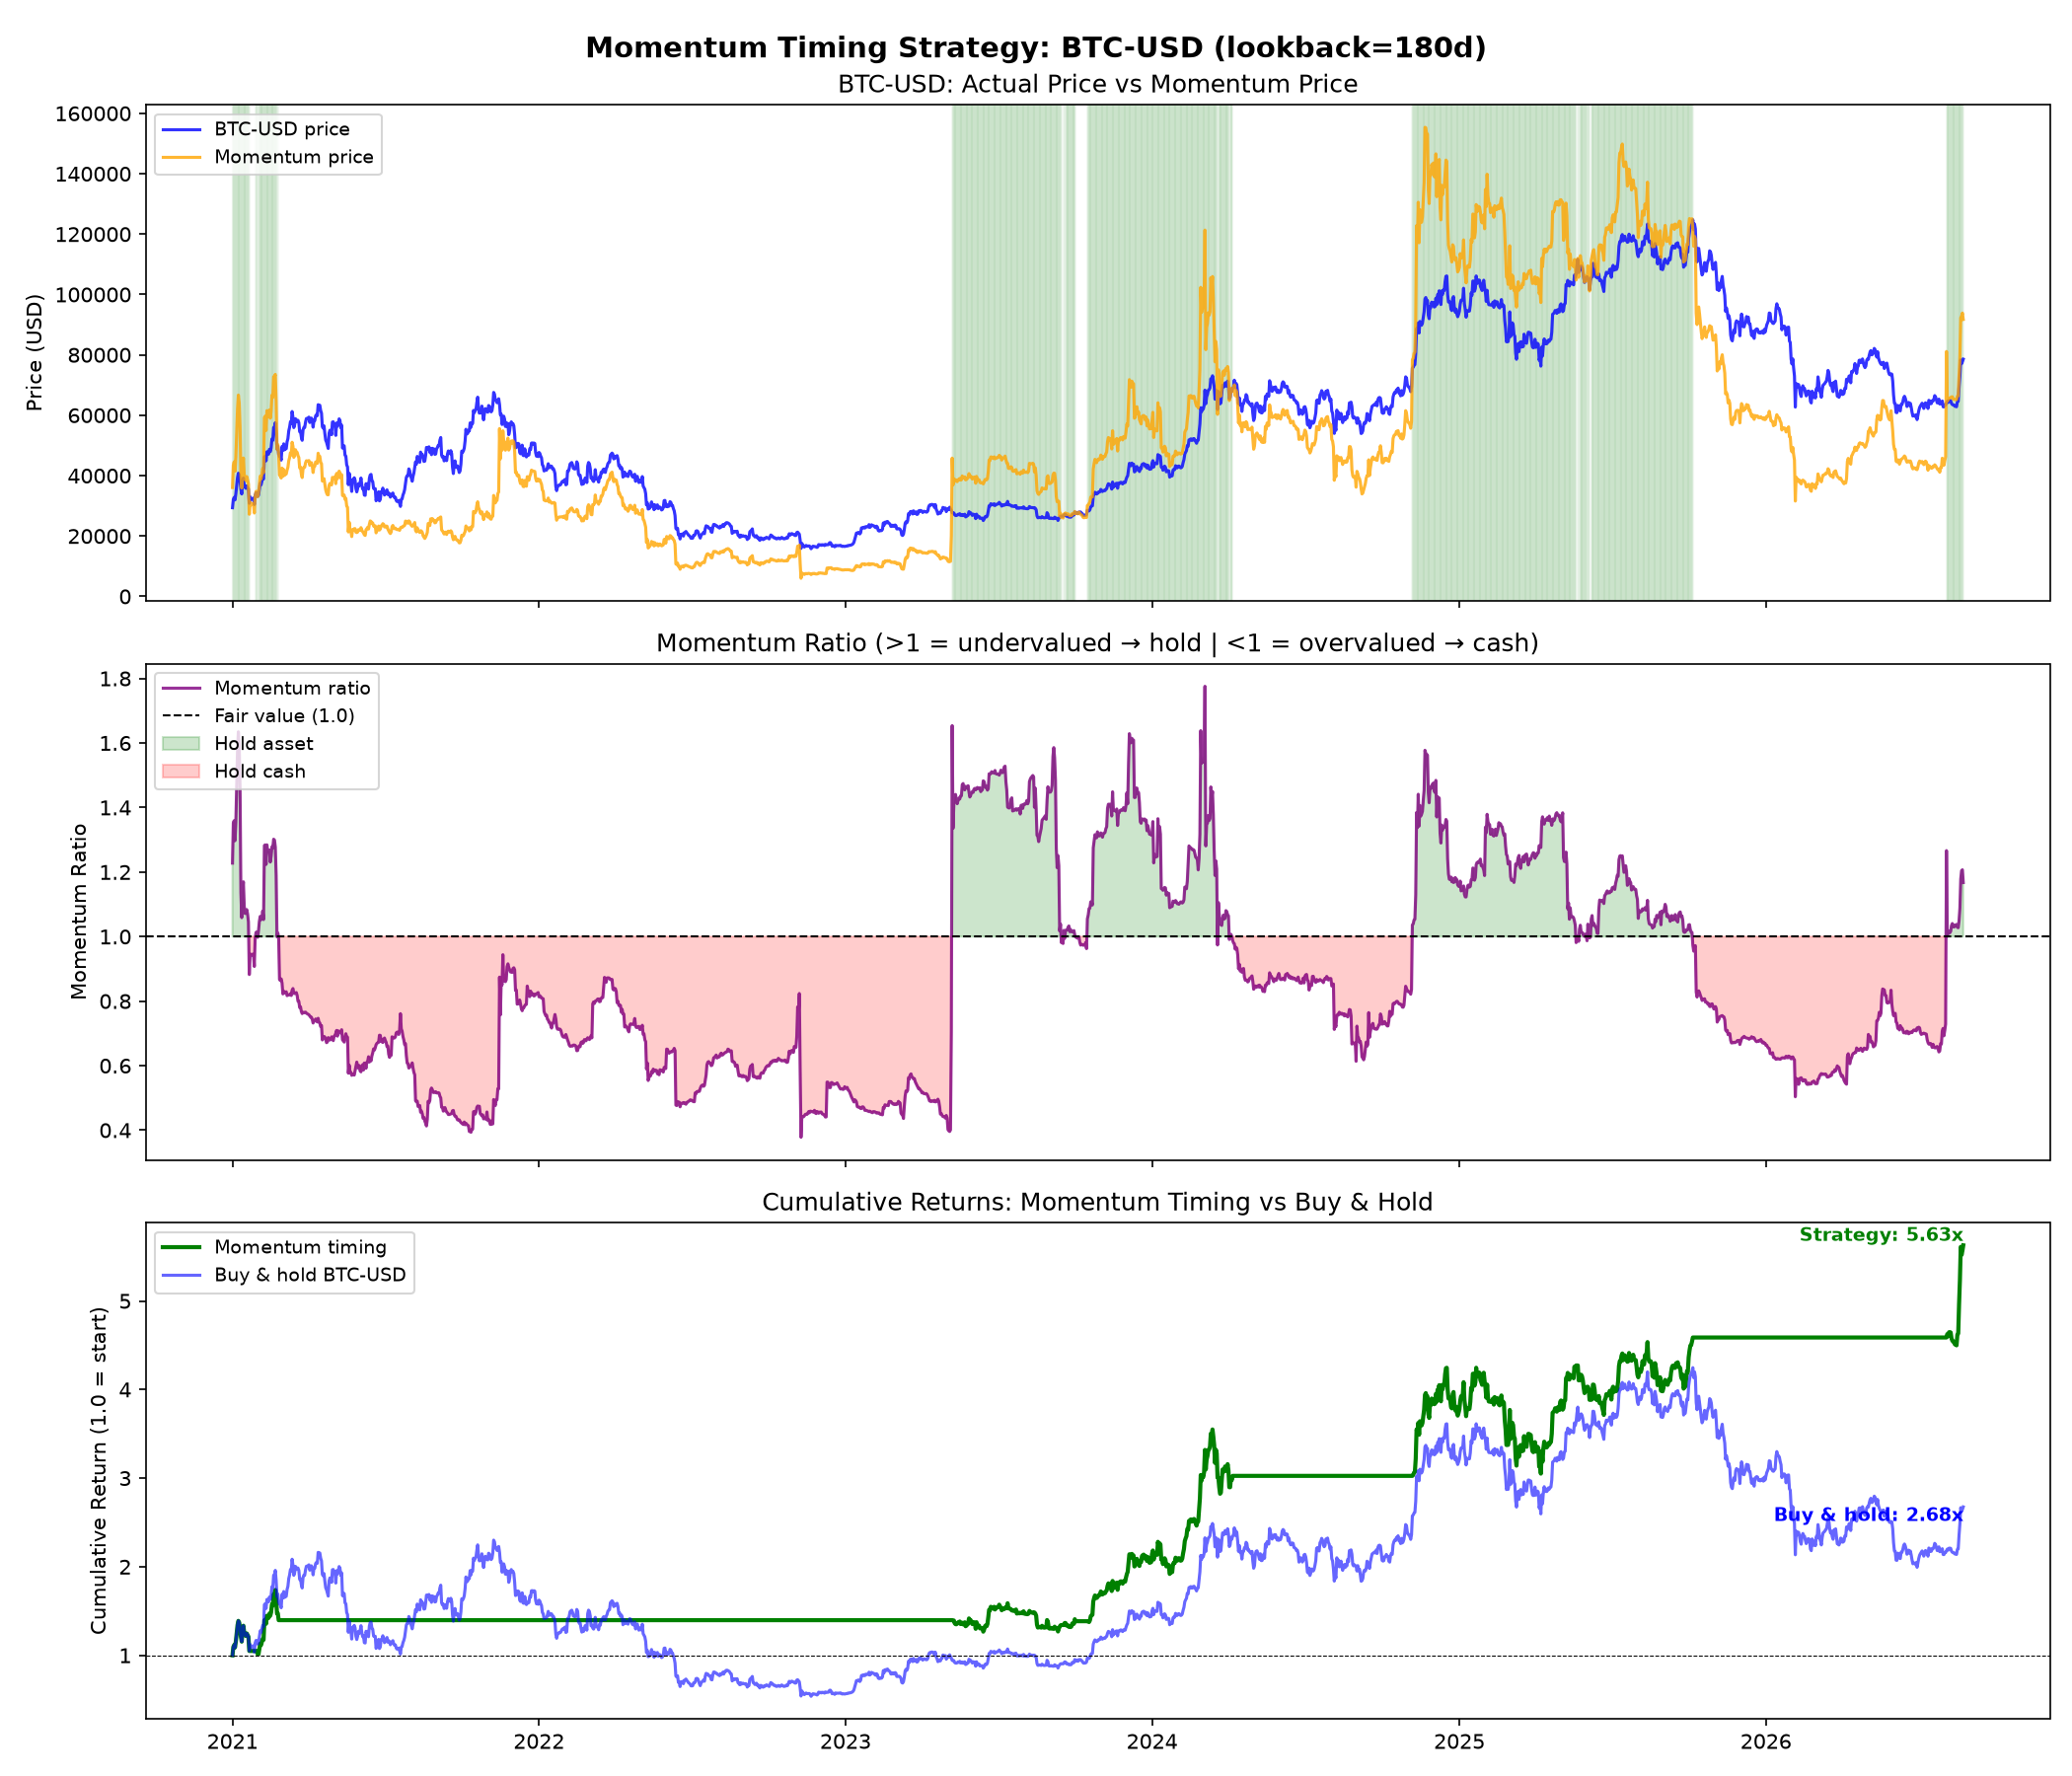
\includegraphics[width=\textwidth]{timing_BTCUSD.png}
    \caption{Top: BTC price (blue) vs momentum price (orange), with
    green shading when the strategy holds BTC. Middle: momentum ratio
    with hold/cash zones. Bottom: cumulative returns --- strategy
    (green) vs buy \& hold (blue). The strategy reaches 5.63x vs
    2.68x for buy \& hold.}
\end{figure}

Key observations from the chart:

\begin{enumerate}[leftmargin=2em]
    \item The strategy \textbf{exits before the 2022 crash} ---
          the momentum ratio drops below 1.0 as volume flows turn
          negative, signalling that the pool of money no longer
          supports the price.
    \item It \textbf{re-enters during the 2023 accumulation phase},
          when volume flows quietly turn positive while the price is
          still depressed.
    \item It \textbf{rides the 2024--2025 bull run} but exits during
          corrections, preserving gains.
    \item The strategy spends two thirds of its time in cash,
          dramatically reducing stress and exposure.
\end{enumerate}

%% ── LOOKBACK SENSITIVITY ─────────────────────────────────────────

\section{Lookback Window Sensitivity}

\begin{itemize}[leftmargin=2em]
    \item \textbf{90 days}: Too reactive. Generates 22 trades with a
          45\% win rate. Gets whipsawed by short-term volatility.
          Average losses (-9.2\%) are too large relative to wins
          (+14.8\%).
    \item \textbf{180 days}: The sweet spot. 16 trades, 62\% win rate.
          Captures the major trend shifts (bear market entry/exit, bull
          market participation) without overtrading. The win/loss
          asymmetry (+26.8\% vs -1.9\%) is exceptional.
    \item \textbf{365 days}: Too slow. Only 10 trades. Enters late and
          exits late. Still beats cash (+132.3\%) and dramatically
          reduces drawdown (-33.2\% vs -76.6\%), but misses the best of
          the moves. Returns to +132\% vs buy \& hold's +167\%.
\end{itemize}

\textbf{Interpretation}: Bitcoin has a roughly 6-month momentum cycle.
The 180-day window aligns with this natural rhythm --- long enough to
filter noise, short enough to catch regime changes. This is consistent
with the ASX backtest, which also used 6-month (182-day) evaluation
periods.

%% ── CAVEATS ──────────────────────────────────────────────────────

\section{Caveats and Risks}

\begin{enumerate}[leftmargin=2em]
    \item \textbf{Backtest $\neq$ live trading.} These results assume
          you can trade at the daily close price with no slippage,
          no fees, and no delay. Real execution will be worse.

    \item \textbf{Small sample.} 16 trades over 5 years is not
          statistically robust. The 62\% win rate could easily be
          50\% or lower out of sample. The strong alpha is driven
          by a few large wins (the 2022 crash avoidance, the 2024
          re-entry).

    \item \textbf{Volume data quality.} The algorithm depends on
          volume reflecting genuine directional conviction. Crypto
          exchanges are known for wash trading (inflating volume
          for rankings). The yfinance data aggregates across
          exchanges, which helps, but the signal may be noisier
          than on regulated equity markets.

    \item \textbf{No transaction costs.} Each trade would incur
          exchange fees (typically 0.1--0.5\% per trade on Kraken).
          With 16 trades (32 transactions), this costs roughly
          3--16\% over the period. This reduces but does not
          eliminate the alpha.

    \item \textbf{Tax implications.} Each exit from BTC is a
          taxable event. Frequent trading creates short-term
          capital gains, taxed at your marginal rate. Buy \& hold
          defers tax until sale and may qualify for the 50\% CGT
          discount (held > 12 months) in Australia.

    \item \textbf{Survivor bias.} We tested BTC \emph{because we
          know it went up}. We would not have tested a coin that
          went to zero. The strategy's apparent success on BTC may
          partly reflect our choice of a winning asset.

    \item \textbf{Regime change.} Bitcoin's market structure is
          evolving (ETF inflows, institutional custody, regulatory
          frameworks). The volume dynamics that produced this signal
          in 2021--2026 may not persist.
\end{enumerate}

%% ── CONCLUSION ───────────────────────────────────────────────────

\section{Conclusion}

The bookmaker pool model, applied as a \textbf{single-asset timing
signal on Bitcoin} with a \textbf{180-day lookback window}, produced
strong results in backtest: +462.7\% return, +295.2\% alpha over buy
\& hold, Sharpe ratio of 1.16, and max drawdown of -28.1\% (vs -76.6\%
for buy \& hold). The strategy is in the market only 34\% of the time.

The \textbf{pairs trade} (BTC/ETH relative value) failed completely
and is abandoned.

The \textbf{ETH single-asset timing} was mediocre and is not
recommended.

\subsection{Next Steps}

\begin{enumerate}[leftmargin=2em]
    \item \textbf{Paper trade.} Run the 180-day BTC signal in
          real-time (no real money) for 3--6 months to see if the
          signal quality holds out of sample.
    \item \textbf{Test on other lookback windows} around 180
          (150, 200, 210) to check sensitivity more finely.
    \item \textbf{Add transaction costs and slippage} to the
          simulation for more realistic results.
    \item \textbf{If paper trading confirms the signal:} open a
          Kraken account, deposit a small amount of BTC, and run
          the strategy live with real money using the CCXT Python
          library for execution.
\end{enumerate}

\vspace{2em}
\begin{center}
\textit{--- Robin}
\end{center}

\newpage
\appendix

\section{Source Code}

\subsection{Core Algorithm: Bookmaker Pool with Rolling Window}

\begin{codebox}[momentum\_single.py --- compute\_rolling\_momentum()]
\begin{lstlisting}[style=python]
def compute_rolling_momentum(history, lookback_days):
    """
    Compute rolling momentum price using the bookmaker pool model.

    Volume is normalised (divided by window mean) to prevent overflow
    on crypto's enormous trade volumes.

    Returns DataFrame with columns: Close, MomentumPrice, MomentumRatio.
    """
    closes = history["Close"].values
    volumes = history["Volume"].values
    dates = history.index

    momentum_prices = [np.nan] * len(history)
    momentum_ratios = [np.nan] * len(history)

    for i in range(lookback_days, len(history)):
        window_close = closes[i - lookback_days:i + 1]
        window_vol = volumes[i - lookback_days:i + 1]

        if len(window_close) < 10:
            continue

        # Daily returns
        returns = np.diff(window_close) / window_close[:-1]
        vols = window_vol[1:]

        # Normalise volume to prevent overflow
        mean_vol = vols.mean()
        if mean_vol == 0:
            continue
        norm_vols = vols / mean_vol

        # Net flow = normalised_volume * return
        net_flows = norm_vols * returns

        # Run the bookmaker pool
        pool = float(window_close[0])
        mp = pool

        for j in range(len(net_flows)):
            pool += net_flows[j] * mp
            mp = pool

        momentum_prices[i] = mp
        momentum_ratios[i] = mp / closes[i]

    result = pd.DataFrame({
        "Close": closes,
        "MomentumPrice": momentum_prices,
        "MomentumRatio": momentum_ratios,
    }, index=dates)

    return result.dropna()
\end{lstlisting}
\end{codebox}

\subsection{Trading Simulation}

\begin{codebox}[momentum\_single.py --- simulate\_timing()]
\begin{lstlisting}[style=python]
def simulate_timing(asset_symbol, lookback_days, start_date, end_date):
    """
    Simulate the timing strategy.

    Rule:
      - If MomentumRatio > 1.0: hold the asset
      - If MomentumRatio <= 1.0: hold cash

    Uses previous day's signal (can't trade on today's close).
    """
    fetch_start = start_date - timedelta(days=lookback_days + 60)

    ticker = yf.Ticker(asset_symbol)
    hist = ticker.history(start=fetch_start, end=end_date, interval="1d")

    df = compute_rolling_momentum(hist, lookback_days)

    # Trim to simulation period
    start_ts = pd.Timestamp(start_date)
    if df.index.tz is not None:
        start_ts = start_ts.tz_localize(df.index.tz)
    df = df[df.index >= start_ts]

    # Signals: 1 = hold asset, 0 = hold cash
    df["signal"] = (df["MomentumRatio"] > 1.0).astype(int)

    # Position: use previous day's signal (no lookahead)
    df["position"] = df["signal"].shift(1).fillna(0).astype(int)

    # Returns
    df["asset_return"] = df["Close"].pct_change().fillna(0)
    df["strategy_return"] = df["position"] * df["asset_return"]

    # Cumulative
    df["cumulative_asset"] = (1 + df["asset_return"]).cumprod()
    df["cumulative_strategy"] = (1 + df["strategy_return"]).cumprod()

    return df
\end{lstlisting}
\end{codebox}

\subsection{Failed Pairs Trade Algorithm (for reference)}

\begin{codebox}[momentum\_crypto.py --- pairs trade signal generation]
\begin{lstlisting}[style=python]
def compute_momentum_price(history):
    """
    Bookmaker model adapted for crypto (single window).
    Volume normalised to prevent overflow.
    """
    h = history.copy()
    h["DailyReturn"] = h["Close"].pct_change()

    mean_vol = h["Volume"].mean()
    if mean_vol == 0:
        return None
    h["NormVolume"] = h["Volume"] / mean_vol
    h["NetVolumeFlow"] = h["NormVolume"] * h["DailyReturn"]
    h = h.dropna()

    pool = float(h["Close"].iloc[0])
    mp = pool
    momentum_prices = [mp]

    for i in range(1, len(h)):
        net_flow = float(h["NetVolumeFlow"].iloc[i])
        pool += net_flow * mp
        mp = pool
        momentum_prices.append(mp)

    return pd.Series(momentum_prices, index=h.index,
                     name="MomentumPrice")


# Signal generation for pairs trade:
# BUY base (sell quote) when base undervalued AND quote overvalued
df["signal"] = 0
df.loc[
    (df["base_momentum_ratio"] > 1 + threshold) &
    (df["quote_momentum_ratio"] < 1 - threshold),
    "signal"
] = 1   # long base / short quote

df.loc[
    (df["base_momentum_ratio"] < 1 - threshold) &
    (df["quote_momentum_ratio"] > 1 + threshold),
    "signal"
] = -1  # short base / long quote
\end{lstlisting}
\end{codebox}

\subsection{Running the Backtest}

\begin{codebox}[Shell commands]
\begin{lstlisting}[style=python,language=bash,keywordstyle=\color{codekw}]
# Setup
cd ~/git/andy/crypto
python3 -m venv venv
source venv/bin/activate
pip install yfinance pandas numpy matplotlib

# Single-asset timing (the one that works)
python momentum_single.py --asset BTC-USD --lookback 180 --plot

# Pairs trade (the one that doesn't)
python momentum_crypto.py --base ETH-USD --quote BTC-USD \
       --threshold 0.01 --plot

# Try different lookback windows
python momentum_single.py --asset BTC-USD --lookback 90 --plot
python momentum_single.py --asset BTC-USD --lookback 365 --plot

# Custom date range
python momentum_single.py --asset BTC-USD --lookback 180 \
       --start 2020-01-01 --end 2026-08-24 --plot
\end{lstlisting}
\end{codebox}

\end{document}
